In this section we present a detailed computational study of the automated
goal-oriented adaptive algorithm presented in \autoref{sec:Algorithm} applied to
some time-dependent test problems. To this end we first we apply our algorithm
to a linear problem, \autoref{tst:Heat}, where the error representation is
orthogonal due to Galerkin orthogonality. Namely, we demonstrate the
effectiveness of \autoref{alg:Adaptivity} on the heat equation. Next we
demonstrate the effectiveness of \autoref{alg:Adaptivity} on non-linear
problems, where the error representation is no longer orthogonal. To this end,
we apply the algorithm to a benchmark problem presented in Sch\"afer et
al.\cite{Schaefer1996}, \autoref{tst:Cylinder2D}, where the equation of interest
is the Icompressible Navier-Stokes equation and our particular focus is on flow
around a bluff body.  Finally, in \autoref{tst:rhoNSE}, we apply our algorithm
to the ever more complex problem of Variable Density Incompressible
Navier-Stokes equation, where we focus on the solution to Rayleigh-Taylor
instability.

For each test below we set the max iteration to $20$ and set the $TOL=0$. In
this way we will treat the solution obtained from the final adaptive mesh as the
so-called 'true solution' and use this solution to determine the effectivity of
the adaptive algorithm.

\subsection{Orthogonal Error Representation}
In this subsection we demonstrate the effectiveness of \autoref{alg:Adaptivity}
for problems where the global error representation is orthogonal. In these types
of problems the traditional thought is that the error representation doesn't
provide information about the error. However, in \autoref{tst:Heat}, we show
that the local error representation does, indeed, contain significant
information about the error and thus is an effective way of controlling the
error.

\begin{test}[Anisotropic Heat Equation] \label{tst:Heat}
  The heat equation is a purely parabolic linear partial differential equation
  and therefore the global error representation is zero due to Galerkin
  Orthogonality.  Thus it is an excellent choice to demonstrate the
  effectiveness of the algorithm described in \autoref{sec:Algorithm}.

  In this test problem we extend the test given by Li et al.
  \cite[Example 5.1]{Li2010}, i.e. the anisotropic diffusion equation, to the
  time dependent case. Thus we are concerned with the numerical solution of the
  anisotropic heat equation on a domain with a hole given by
  \begin{equation} \label{eqn:Heat}
    \begin{split}
      u_t - \nabla \cdot (\kappa \nabla u) &= f, \quad \text{in } \Omega \\
      u &= g, \quad \text{on } \partial \Omega \\
      u(x,y,0) &= u_0(x,y)
    \end{split}
  \end{equation}
  where $\Omega = \Omega_1\setminus~\Omega_2$ is the physical domain, $f$ is the
  forcing function, $g$ is the function describing the boundary condition, and
  $\kappa$ is the diffusion tensor. For this test we take $\Omega_1 = [0,
  1]^2$, $\Omega_2 = [\frac{4}{9}, \frac{5}{9}]^2$, $f = 0$
  \begin{equation}
    g = \begin{cases}
        0 & \text{if } (x,y) \in \partial \Omega_1 \\
        0.5 - 0.5\, \cos(10\, t) & \text{if } (x,y) \in \partial \Omega_2,
    \end{cases}
    \label{eqn:BCFunction}
  \end{equation}
  and the diffusion tensor to be
  \begin{equation}
    \kappa = \begin{bmatrix} 500.5 & 499.5 \\ 499.5 & 500.5 \end{bmatrix}.
    \label{eqn:DiffusionTensor}
  \end{equation}
  The above diffusion tensor results in a diffusion process which is
  preferential along the line $x = y$.

  Taking $u^n \in H^1_g(\Omega)$ and applying a cG(1) finite element
  discretization, i.e. piecewise linear test and trial functions, with implicit
  Euler time-stepping to \eqref{eqn:Heat} results in the following weak residual
  \begin{equation}
    r(u^n, v) = (u^n - u^{n-1})\, k^{-1} + (\kappa \nabla u^n, \nabla v)
      - (f, v) = 0, \quad \forall v \in H^1_0(\Omega)
    \label{eqn:HeatWeak}
  \end{equation}
\end{test}

\subsection{Non-Orthogonal Error Representation}
In this subsection we demonstrate the effectiveness of \autoref{alg:Adaptivity}
applied to problems where the global error representation is no longer
orthogonal. In particular, we look at applying \autoref{alg:Adaptivity} to the
Incompressible Navier-Stokes and the Variable Density Incompressible Navier
Stokes. In both cases, we solve each test case using a
Galerkin\slash~Least-Squares (GLS) stabilized cG(1)cG(1) finite element, where
the first cG(1) indicates that the test and trial functions are both piecewise
linear, while the second cG(1) indicates that the test piecewise constants and
the trial functions are continuous piecewise linear.

\subsubsection{Incompressible Navier-Stokes}
For the test problem \ref{tst:Cylinder2D} we are concerned with the
Incompressible Navier-Stokes with constant kinematic viscosity, $\nu>0$, in a
domain $\Omega\subset \R^d$, with boundary $\partial \Omega$, i.e.  where the
strong residual is given by
\begin{equation}
    \begin{split}
      \mathbf{u}_t + \left( \mathbf{u} \cdot \nabla \right) \mathbf{u} - \nu\,
          \Delta \mathbf{u} + \nabla p = \mathbf{f}, \quad \mathbf{x} \in \Omega \\
          \nabla \cdot \mathbf{u} = 0, \quad \mathbf{x} \in \Omega
    \end{split}
  \label{eqn:NSE}
\end{equation}
Given a step size $k$ and applying the cG(1)cG(1) finite element discretization
to \autoref{eqn:NSE} with $V = (v, q) \in X \subset [H^1_0(\Omega)]^d \times
H^1(\Omega)$ gives the following weak residual
\begin{equation}
  \begin{split}
    r(\bar{U}^n; V) &= \left(\mathbf{u}^n - \mathbf{u}^{n-1}, v\right)\,k^{-1}
        + (\left( \bar{\mathbf{u}}^n \cdot \nabla \right) \bar{\mathbf{u}}^n, v) \\
        &\quad+ \nu\, (\nabla \bar{\mathbf{u}}^n, \nabla v)
        - (p^n, \nabla \cdot v) - (\mathbf{f}, v)
        + (\nabla \cdot \bar{\mathbf{u}}^n, v) = 0
  \end{split}
  \label{eqn:WeakNSE}
\end{equation}
where $\bar{U}^n = (\bar{\mathbf{u}}^n,p)$, and $\bar{\mathbf{u}}^n =
\frac{1}{2}\left(\mathbf{u}^n + \mathbf{u}^{n-1}\right)$. Given the solution
$U=(\mathbf{u},p)$, since the elements we are concerned with (cG(1)cG(1)) have
test functions which are linear in space and constant in time the strong
residual is given by
\begin{equation}
    R(\bar{U}^n,U) = \begin{cases}
      \left(\mathbf{u} \cdot \nabla \right) \bar{\mathbf{u}}^n
        + \nabla p^n - \mathbf{f} = 0 \\
      \nabla \cdot \bar{\mathbf{u}}^n = 0.
    \end{cases}
  \label{eqn:StrongNSE}
\end{equation}
Finally, the GLS-cG(1)cG(1) discretization of \eqref{eqn:NSE} is given by
\begin{equation}
  r(\bar{U}^n,V) + SD_{\delta}^n(\bar{U}^n,V) = 0, \quad \forall V=(v,q) \in X.
  \label{eqn:G2}
\end{equation}
Here $SD_{\delta}^n$ is the GLS and is given by
\begin{equation}
  SD_{\delta}^n \equiv
    \delta_1 (\left(\bar{\mathbf{u}}^n \cdot \nabla \right) \bar{\mathbf{u}}^n
        + \nabla p^n - \mathbf{f},
      \left(\bar{\mathbf{u}}^n \cdot \nabla \right) v + \nabla q)
      + \delta_2 (\nabla \cdot \bar{\mathbf{U}}^n, \nabla \cdot v),
  \label{eqn:NSEStabilization}
\end{equation}
where $\delta_1 = \kappa_1 (k^{-1} + |\mathbf{u}^{n-1}|^2\, h^{-2})^{-1/2}$, and
$\delta_2 = \kappa_2 h$, while $\kappa_1$ and $\kappa_2$ are problem independent
constants of unit size. For each test case below we take the time-step to be
\begin{equation*}
  k = C_{CFL}\, \frac{\min_{\mathcal{T}_K}(h)}{|U_m|},
\end{equation*}
where $C_{CFL}=100$.

\begin{test}[Flow Around a Cylinder] \label{tst:Cylinder2D}
  This test case is based on a benchmark problem from Sch\"afer and Turek
  \cite[Test case 2D-2]{Schaefer1996}. Thus, we define the domain to be a
  rectangular domain with a circle removed (see \autoref{fig:2DCylinder}). For
  the inlet boundary condition we take
  \begin{equation}
    u(0,y,t) = (4\, U_m\,y\, (H - y)/H^2, 0),
    \label{eqn:2DInlet}
  \end{equation}
  where $U_m = 1.5\, \text{m/s}$, $H = 0.41\, \text{m}$. For the kinematic
  viscosity we take $\nu = 10^{-3}\, \text{m}^2\text{/s}$, resulting in a
  Reynolds number of $Re=100$.

  \begin{figure}[h]
    \centering
    \tikzstyle{next}=[->, thick, shorten <=1pt, shorten >=1pt]
    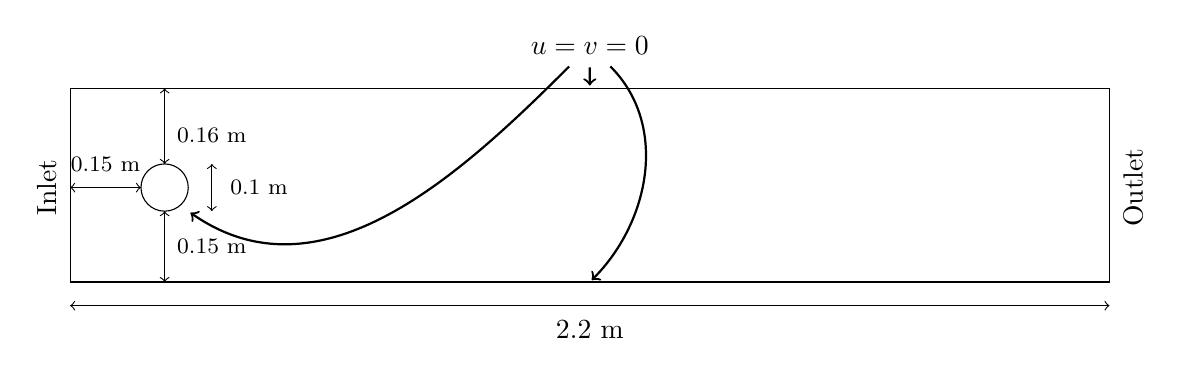
\begin{tikzpicture}[scale=6]
        \draw (0,0) -- (2.2,0) -- (2.2,0.41) -- (0,0.41) -- cycle;
        \draw (0.2,0.2) circle (0.05);
        \draw[<->] (0,-0.05) -- (2.2,-0.05);
        \draw (1.1,-0.1) node {2.2 m};
        \draw[<->] (0,0.2) -- (0.15,0.2);
        \draw (0.075,0.25) node {\footnotesize 0.15 m};
        \draw[<->] (0.2,0) -- (0.2,0.15);
        \draw (0.3,0.075) node {\footnotesize 0.15 m};
        \draw[<->] (0.2,0.25) -- (0.2,0.41);
        \draw (0.3,0.31) node {\footnotesize 0.16 m};
        \draw[<->] (0.3,0.15) -- (0.3,0.25);
        \draw (0.4,0.2) node {\footnotesize 0.1 m};
        \node[rotate=90] (outflow) at (2.25, 0.2) {Outlet};
        \node[rotate=90] (inflow) at (-0.05, 0.2) {Inlet};
        \node (NoFlow) at (1.1,0.5) {$u=v=0$};
        \draw[next] (NoFlow) to (1.1,0.41);
        \draw[next] (NoFlow) to [out=-45,in=45] (1.1,0);
        \draw[next] (NoFlow) to [out=-135,in=-35] (0.25,0.15);
    \end{tikzpicture}
    \caption{Geometry of \autoref{tst:Cylinder2D}}
    \label{fig:2DCylinder}
  \end{figure}
\end{test}

\subsubsection{Variable Density Incompressible Navier-Stokes}
In this subsection we again will demonstrate the effectiveness of
\autoref{alg:Adaptivity}, but this time we apply the algorithm to a density
dependent problem. More specifically, in \autoref{tst:rhoNSE} we look at the
effectiveness of \autoref{alg:Adaptivity} applied to Rayleigh-Taylor instability
modelled by the variable density incompressible Navier-Stokes equations, i.e.
\begin{equation}
    \begin{split}
        &\rho_t + \nabla \cdot \left( \rho \mathbf{u} \right) = 0 \\
        &\rho \left( \mathbf{u}_t
            + \left( \mathbf{u}\cdot \nabla \right) \mathbf{u} \right)
            - \nu \Delta \mathbf{u} + \nabla p = \rho\, \mathbf{f} \\
        &\nabla \cdot \mathbf{u} = 0,
    \end{split}
    \label{eq:DensityNSE}
\end{equation}
where $\rho$ is the fluid density, $\mathbf{u} = \left[ u, v \right]^T$ is the
fluid velocity in 2D, $p$ is the fluid pressure, $\mathbf{f}$ is the
external forcing, and $\nu$ is the kinematic viscosity.

Again, we take a step size of $k$ and apply the cG(1)cG(1) finite
element to \autoref{eq:DensityNSE}, however this time we use a different
stabilization scheme. For the variable density Navier-Stokes equations we
choose to use artificial viscosity as our stabilization scheme. Thus, taking
$V = (v, q, \chi) \in X = \left[ H^1_0(\Omega) \right]^2 \times H^1(\Omega)
\times H^1(\Omega)$ results in the following weak residual
\begin{equation}
    \begin{split}
        r(\bar{U}^n; V) &= (\rho^n - \rho^{n-1}, \chi) + (\nabla \cdot \left(
            \rho \mathbf{u} \right), \chi) \\
        &+  \rho\, \left(\left(\mathbf{u}^n
                - \mathbf{u}^{n-1}, v\right)\,k^{-1}
            + (\left( \bar{\mathbf{u}}^n \cdot \nabla \right)
                \bar{\mathbf{u}}^n, v)\right)
            + \nu\, (\nabla \bar{\mathbf{u}}^n, \nabla v)
            - (p^n, \nabla \cdot v) - \rho\, (\mathbf{f}, v) \\
        &+ (\nabla \cdot \bar{\mathbf{u}}^n, v) = 0
    \end{split}
    \label{eq:WeakRhoNSE}
\end{equation}

\begin{test}[Variable Density Navier-Stokes] \label{tst:rhoNSE}
\end{test}
